\begin{titlepage}
	
	\includepdf[noautoscale=False,fitpaper=True]{thesis-cover/thesis-cover.pdf}
%\pagecolor{mDarkTeal}\afterpage{\nopagecolor}
%{\color{mLightBrown}%\afterpage{\notextcolor}
%\begin{center}
%
%%% Extra whitespace at the top.
%\vspace*{2\bigskipamount}
%
%%% Print the title.
%{\makeatletter
%	\linespread{1.1}
%\titlestyle\bfseries\Huge\@title
%\par
%\makeatother}
%
%%% Print the optional subtitle.
%{\makeatletter
%\ifx\@subtitle\undefined\else
%    \bigskip
%    \titlefont\titleshape\Large\@subtitle
%\fi
%\makeatother}
%
%\vspace{10cm}
%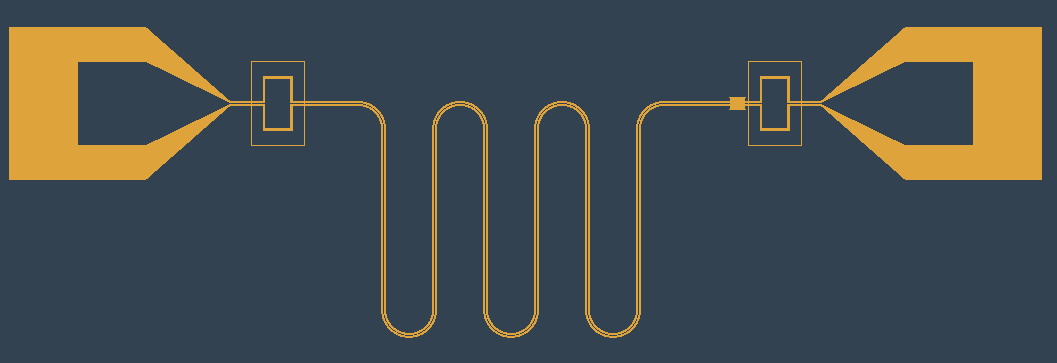
\includegraphics[width=\linewidth]{title/cover_circuit/cover_circuit}
%\end{center}
%
%
%}

%\cleardoublepage
\thispagestyle{empty}

\begin{center}

%% The following lines repeat the previous page exactly.

\vspace*{2\bigskipamount}

%% Print the title.
{\makeatletter
\titlestyle\bfseries\LARGE\@title
\par
\makeatother}

%% Print the optional subtitle.
{\makeatletter
\ifx\@subtitle\undefined\else
    \bigskip
    \titlefont\titleshape\Large\@subtitle
\fi
\makeatother}

%% Uncomment the following lines to insert a vertically centered picture into
%% the title page.
%\vfill
%\includegraphics{title}
\vfill

%% Apart from the names and dates, the following text is dictated by the
%% promotieregelement.

{\Large\titlefont\bfseries Dissertation}

\bigskip
\bigskip

for the purpose of obtaining the degree of doctor

at Delft University of Technology

by the authority of the Rector Magnificus, prof.dr.ir. T.H.J.J. van der Hagen

chair of the Board for Doctorates

to be defended publicly on

%Monday 1 June 2020 at 10:00h

\bigskip
\bigskip

by

\bigskip
\bigskip

%% Print the full name of the author.
\makeatletter
{\Large\titlefont\bfseries\@firstname\ {\titleshape\@lastname}}
\makeatother

\bigskip
\bigskip

Master of Science Nanostructure Technology, \\
Julius-Maximilians-Universität Würzburg, \\
born in Cologne, Germany

%% Extra whitespace at the bottom.
\vspace*{2\bigskipamount}

\end{center}

\clearpage
\thispagestyle{empty}

%% The following line is dictated by the promotieregelement.
\noindent This dissertation has been approved by the promotors.

\bigskip
\noindent Composition of the doctoral committee:

%% List the committee members, starting with the Rector Magnificus and the
%% promotor(s) and ending with the reserve members.
\medskip\noindent
\begin{tabular}{p{3.5cm}l}
    Rector Magnificus, & chairperson \\
    Prof.~Dr.~G.A.~Steele, & Delft University of Technology, promotor \\
    Dr.~A.~Akhmerov, & Delft University of Technology, promotor \\

    \medskip
    \mbox{\emph{Independent members:}} & \\
%	\mbox{\emph{Onafhankelijke leden:}} & \\
    
%    Prof.~Dr.~C.~Schönenberger, & University of Basel, Switzerland \\
%    
%    Prof.~Dr.~P.~Hakonen, & Aalto University, Finland \\
%    
%    Prof.~Dr.~Y.~Blanter, & Delft University of Technology \\
%    
%    Dr.~J.~Prance, & Lancaster University, United Kingdom \\
%
%    Dr.~T.~van~der~Sar, & Delft University of Technology \\
    
%    \medskip
%    \mbox{\emph{Reserve member:}} & \\

%    Prof.~Dr.~H.S.J.~van~der~Zant, & Delft University of Technology \\

    
    % \medskip
    % \mbox{\emph{Overige leden:}} & \\
    % Prof.\ dr.\ ir.\ J.\ de Wit, & Technische Universiteit Delft \\
    % Dr.\ ir.\ Q.\ de Zwart, & Technische Universiteit Eindhoven \\
\end{tabular}

%% Include the following disclaimer for committee members who have contributed
%% to this dissertation. Its formulation is again dictated by the
%% promotieregelement.
% \medskip
% \noindent Prof.\ dr.\ ir.\ J.\ de Wit heeft in belangrijke mate aan de totstandkoming van het proefschrift bijgedragen.

%% Here you can include the logos of any institute that contributed financially
%% to this dissertation.
\vfill
\begin{center}
    \centering
    
\includegraphics[height=0.5in]{title/logos/tudelft}
    \hspace{2em}
    
\includegraphics[height=0.5in]{title/logos/casimir}
    \vspace{0.5cm}\newline
    
\includegraphics[height=0.5in]{title/logos/flagship}
\end{center}
\vfill

\noindent
\begin{tabular}{@{}p{0.2\textwidth}@{}p{0.8\textwidth}}
    \textit{Keywords:} & Graphene, Josephson junctions, Josephson inductance, superconducting microwave circuits, current detection. \\
    \textit{Printed by:} &  Gildeprint. \\
    \textit{Cover:} & Schematic circuit layout for the base layer of a shunt capacitor DC bias cavity.
\end{tabular}

\vspace{4\bigskipamount}

\noindent Copyright \textcopyright\ 2020 by Felix E.~Schmidt

%% Uncomment the following lines if this dissertation is part of the Casimir PhD
%% Series, or a similar research school.
%\medskip
\noindent Casimir PhD Series, Delft-Leiden 2020-05

\medskip
\noindent ISBN 000-00-0000-000-0

\medskip
\noindent An electronic version of this dissertation is available at \\
\url{http://repository.tudelft.nl/TODO:add_link}.

\end{titlepage}

